\documentclass[12pt]{article}
\usepackage[dvips]{epsfig}
\usepackage{fleqn}
\usepackage{amssymb,amstext}
\usepackage{array}
\usepackage[latin1]{inputenc}
\usepackage{amsmath}
\usepackage[margin=1in]{geometry}
\usepackage{array}
\usepackage{amsmath}
\usepackage{latexsym}
\usepackage{psfrag}
\usepackage{graphicx}
\usepackage{setspace}
\usepackage{caption2}
\usepackage{url}
\usepackage{fancyhdr}
\usepackage{natbib}
\usepackage{cancel}
\usepackage{hyperref}
\usepackage{enumitem}
\usepackage{pdfpages}
\usepackage{indentfirst}
\usepackage{float}

\usepackage{pdflscape}
\usepackage{multirow}
\usepackage{longtable}

\usepackage{xcolor}

\usepackage{subfiles}
 
\usepackage{blindtext}


%\usepackage[utf8]{inputenc}

\hypersetup{
    colorlinks,
    citecolor=black,
    filecolor=[rgb]{0,0.5,0.5},
    linkcolor=black,
    urlcolor=black
}

\renewcommand\listfigurename{}
\renewcommand{\captionlabelfont}{\bf}
\renewcommand{\captionlabeldelim}{.}
\newcommand{\argmax}{\operatornamewithlimits{argmax}}
\renewcommand{\baselinestretch}{2}
\renewcommand\refname{References}
\newcommand\crule[3][black]{\textcolor{#1}{\rule{#2}{#3}}}

\setcounter{secnumdepth}{0}
\makeatletter

%\providecommand*{\input@path}{}
%\g@addto@macro\input@path{{./level1//}{./level1/level2//}{./level2//}}
%\makeatother

%\renewcommand\section{\@startsection {section}{1}{\z@}%
%                                   {-3.5ex \@plus -1ex \@minus -.2ex}%
%                                   {2.3ex \@plus.2ex}%
%                                   {\centering\normalfont\Large\scshape}}
%\renewcommand\subsection{\@startsection {subsection}{1}{\z@}%
%                                   {-3.5ex \@plus -1ex \@minus -.2ex}%
%                                   {2.3ex \@plus.2ex}%
%                                   {\normalfont\bf}}
\renewcommand*\contentsname{}                                   
\pagenumbering{gobble}                                   
\begin{document}
	\begin{center}
	{\bf \Large \textit{Armillaria Gallica} Gene Analysis Tools}
	\end{center}

%\section{main}
%All the stuff Thomas did:
%\begin{itemize}
%	\item read depth snapshots - check!
%	\item program to find new significant read depth differences - check!
%	\item average read depth stuff - check!
%	\item total number of aligned reads - check!
%	\item program to take mode of reads - check!
%	\item scaffold graphing program - check!
%	\item read depth differences program - check!
%	\item assemblies
%	\item blasting stuff
%	\item RNA verification
%\end{itemize}
%%%%%%%%%%%%%%%%%%%%%%%%%%%%%%%%%%%
%
%	Read Depth Snapshot
%
%%%%%%%%%%%%%%%%%%%%%%%%%%%%%%%%%%%
\section{Read Depth Snapshots}
	In order to gain a understanding of how the locaitons which Hao had determined had notably high read depth the regions Hao identified were graphed. There were approximatly between 2000 and 4000 regions for each of the 15 strains. Although there were many graphs four predomanant types of high read depth regions stood out: Normal, Rectangular, Right skewed, and Left skewed.
\begin{figure}[H]
	\begin{centering}
		\resizebox{40mm}{40mm}{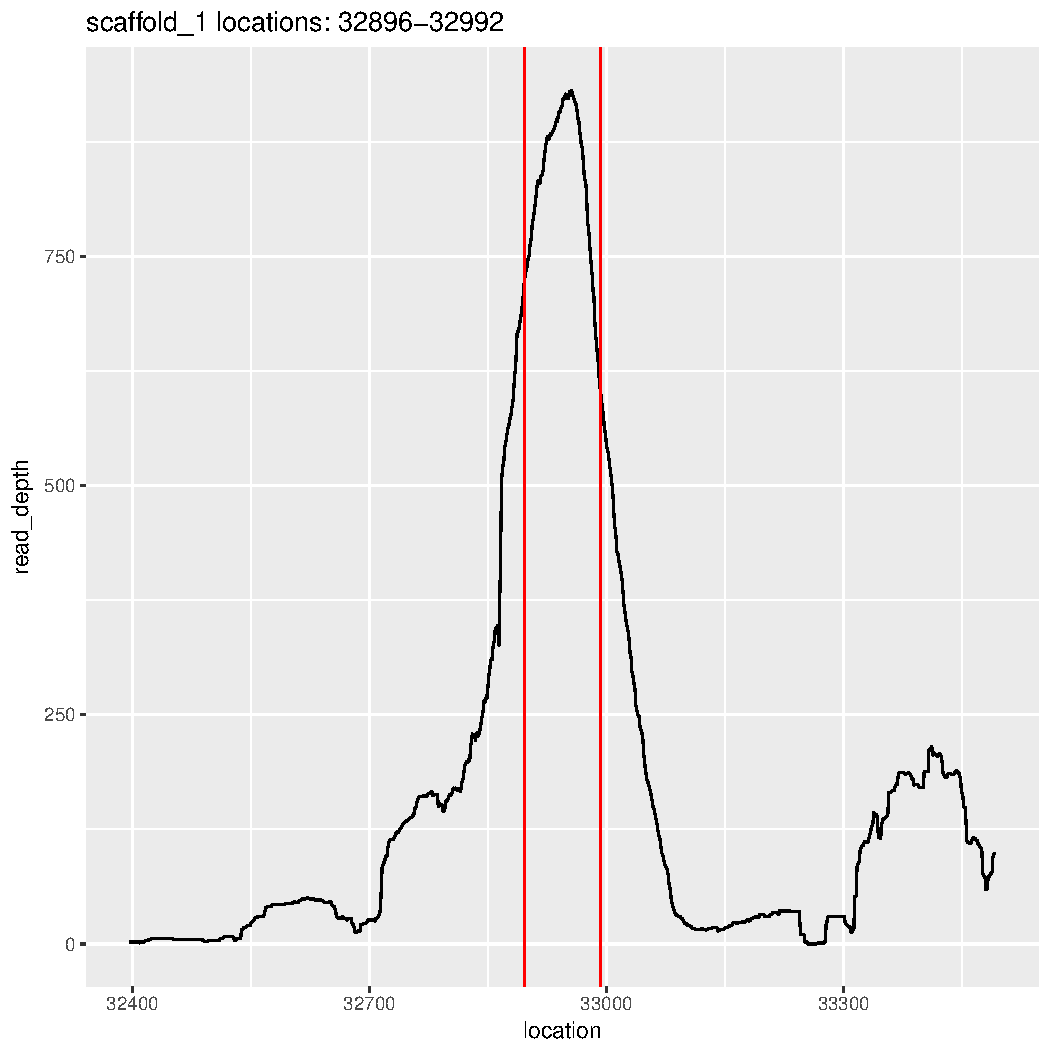
\includegraphics[angle=0,width=1.0\linewidth]{/home/thomas/Directed_Studies_Summer_2019/Armillaria_gallica_gene_analysis_tools/Reporting_documents/Figures/read_depth_snapshot_images/ctj/0_Ar109_read_depth.pdf}}
		\resizebox{40mm}{40mm}{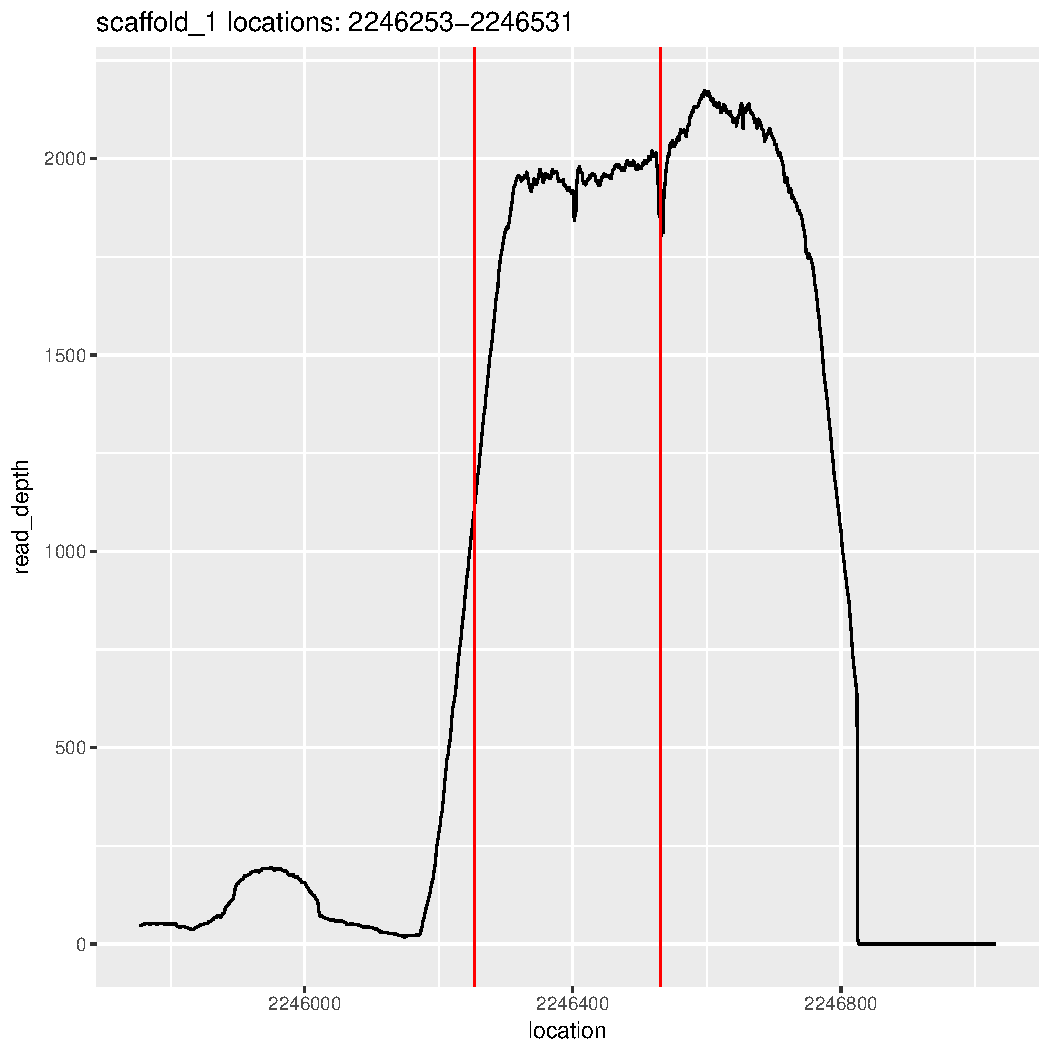
\includegraphics[angle=0,width=1.0\linewidth]{/home/thomas/Directed_Studies_Summer_2019/Armillaria_gallica_gene_analysis_tools/Reporting_documents/Figures/read_depth_snapshot_images/ctj/5_Ar109_read_depth.pdf}}
		\resizebox{40mm}{40mm}{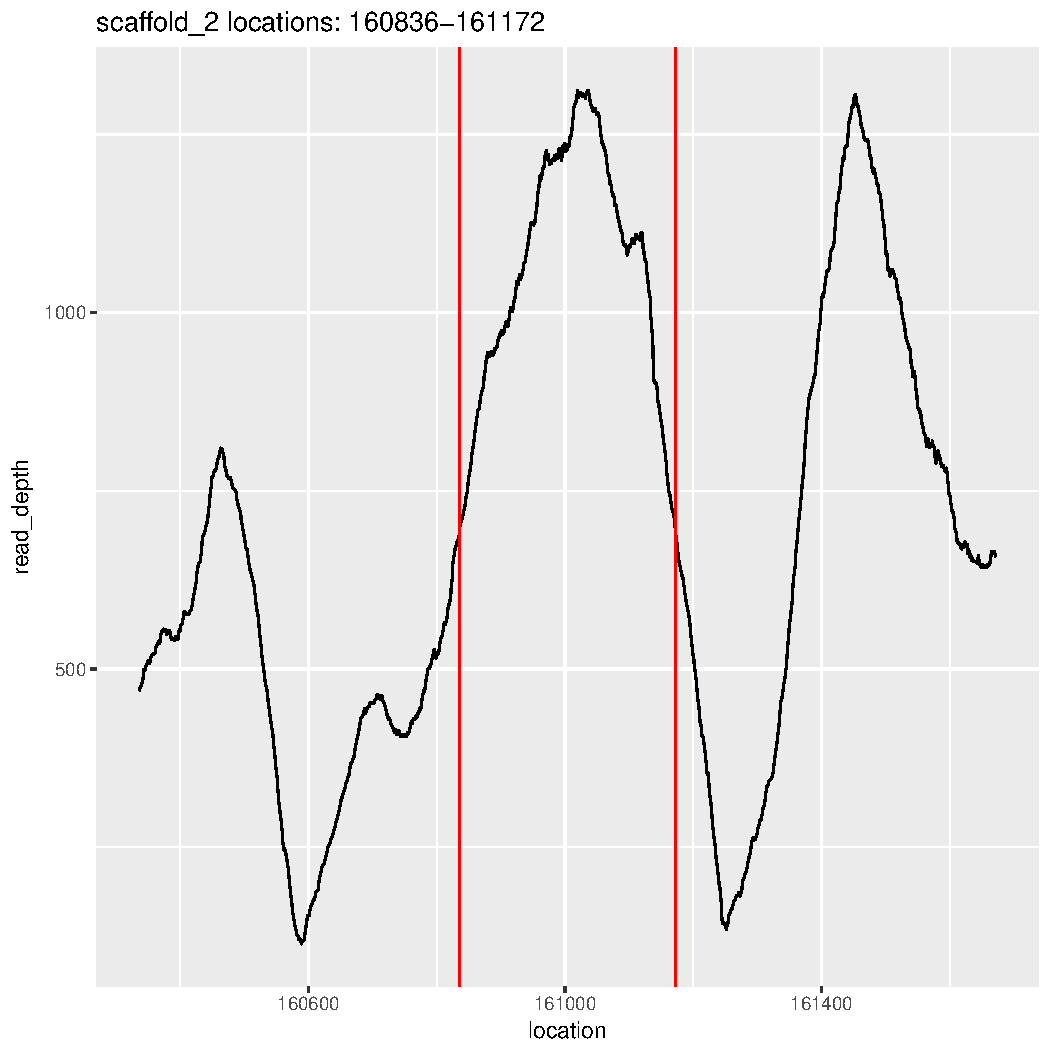
\includegraphics[angle=0,width=1.0\linewidth]{/home/thomas/Directed_Studies_Summer_2019/Armillaria_gallica_gene_analysis_tools/Reporting_documents/Figures/read_depth_snapshot_images/ctj/155_Ar109_read_depth.pdf}}
		\resizebox{40mm}{40mm}{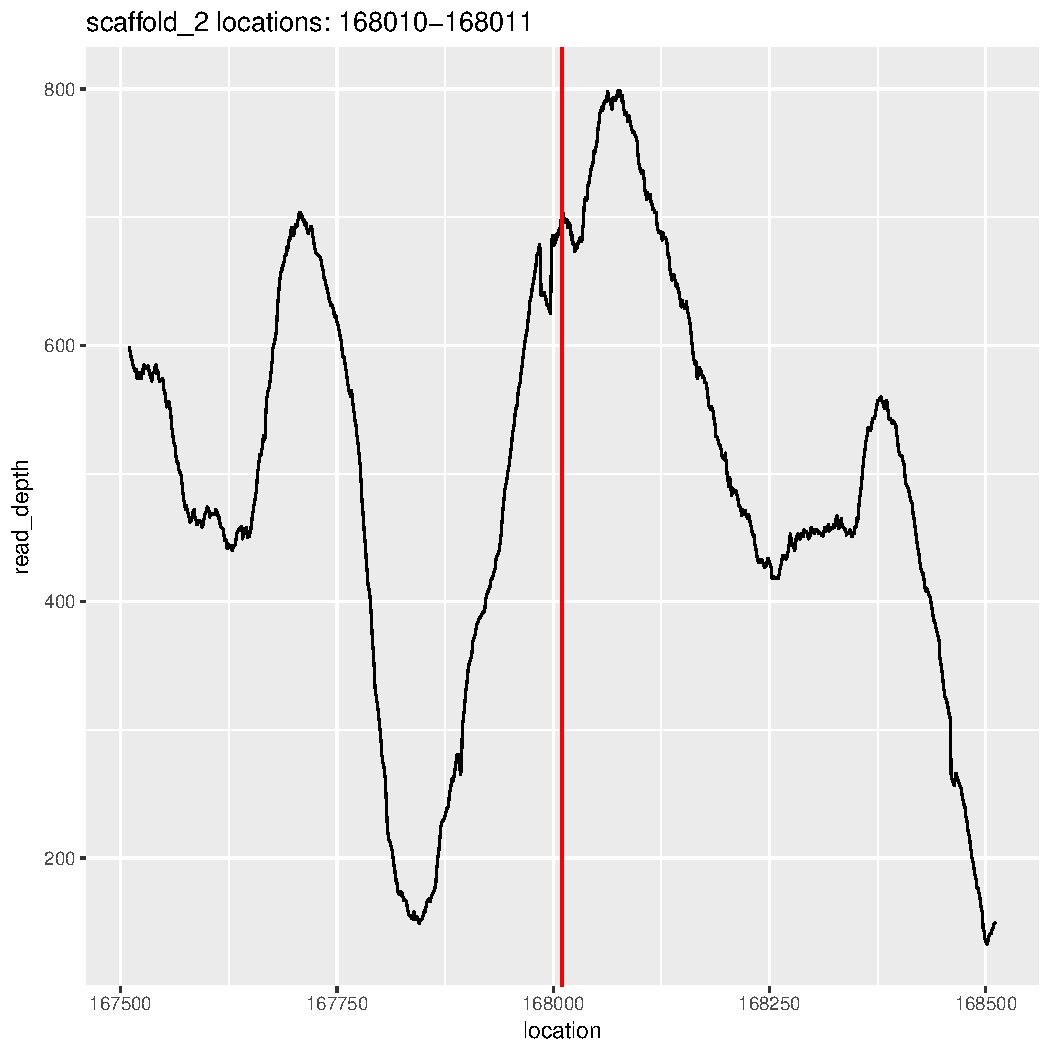
\includegraphics[angle=0,width=1.0\linewidth]{/home/thomas/Directed_Studies_Summer_2019/Armillaria_gallica_gene_analysis_tools/Reporting_documents/Figures/read_depth_snapshot_images/ctj/173_Ar109_read_depth.pdf}}
		\begin{singlespace}
			\vspace{-0.5cm}
			\caption[Examples of the four types of high read depth regions.]{Examples of the four types of high read depth regions (left most) Normal, (left middle) Rectangular, (right middle) Left skewed, (right most)Right skewed}\label{four_rds}
		\end{singlespace}
	\end{centering}
\end{figure}

%%%%%%%%%%%%%%%%%%%%%%%%%%%%%%%%%%%
%
%	Average read depth and total number of reads aligned per scaffold
%
%%%%%%%%%%%%%%%%%%%%%%%%%%%%%%%%%%%
\section{Average Read Depth}
	Due to the large quantity of data present in each bam or fastq file we made use of the meta data of the aligned reads in the form of the average number of aligned reads. We calcualted the average for each strain and scaffold individually, and also calculated the global average read depth. Locations that did not have any reads aligned to them were not taken into accout. The global average read depths are shown in table \ref{globavgrd} and a example of the average read depth per scaffold and the number of aligned reads for each scaffold are graphed in figure \ref{109avgcountgraph}.
\begin{table}[H]
	\begin{center}
		\captionof{table}{Gobal Average Read Depths and Number of Reads for Each Strain} \label{globavgrd}
		\vspace{0.5cm}
		\scalebox{.7}{
		\begin{tabular}{ |c|c|c| }
			\hline
			Strain & Global Average Read Depth & Total Global Number of Reads \\
			\hline
			Ar73 & 111.0507 & 69955093\\
			\hline
			Ar109 & 117.6863 & 70143802\\
			\hline
			Ar119 & 112.4868 & 70015910\\
			\hline
			Ar142 & 109.3741 & 70068064\\
			\hline
			Ar159 & 104.3773 & 69875550\\
			\hline
			Ar170 & 112.3987 & 70033946\\
			\hline
			Ar174 & 113.4283 & 70022954\\
			\hline
			Ar175 & 73.79959 & 69545937\\
			\hline
			Ar176 & 73.21531 & 69583274\\
			\hline
			Ar179 & 117.2196 & 70061598\\
			\hline
			Ar188 & 63.61699 & 68627951\\
			\hline
			Ar194 & 67.88522 & 69488072\\
			\hline
			Ar196 & 113.9182 & 70027951\\
			\hline
			Ar201 & 68.39596 & 69488227\\
			\hline
			Ar213 & 110.9612 & 69988055\\
			\hline
		\end{tabular}
		}
	\end{center}
\end{table}

\begin{figure}[H]
	\begin{centering}

		\resizebox{50mm}{50mm}{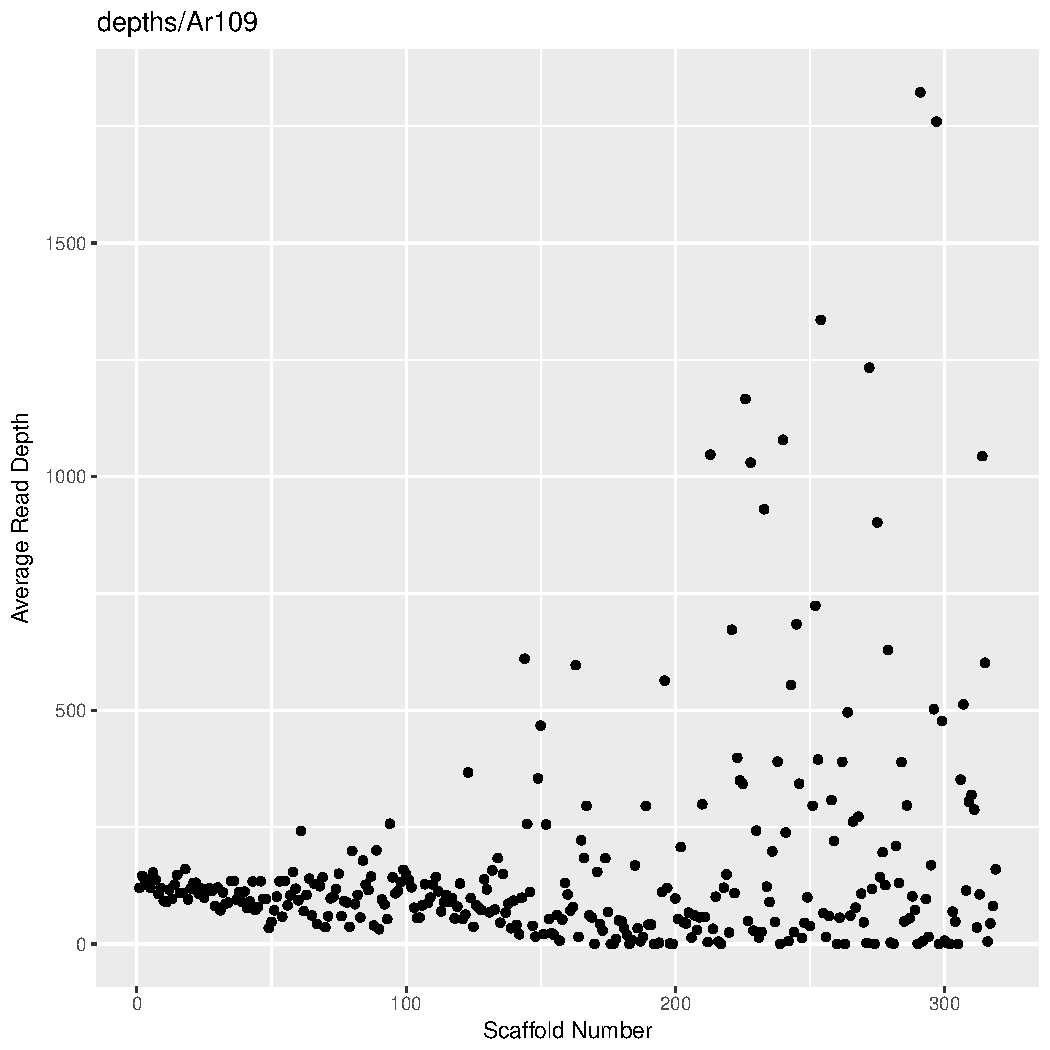
\includegraphics[angle=0,width=1.0\linewidth]{/home/thomas/Directed_Studies_Summer_2019/Armillaria_gallica_gene_analysis_tools/Reporting_documents/Figures/Ar109_collected_no_comma_read_depth.pdf}}
		\resizebox{50mm}{50mm}{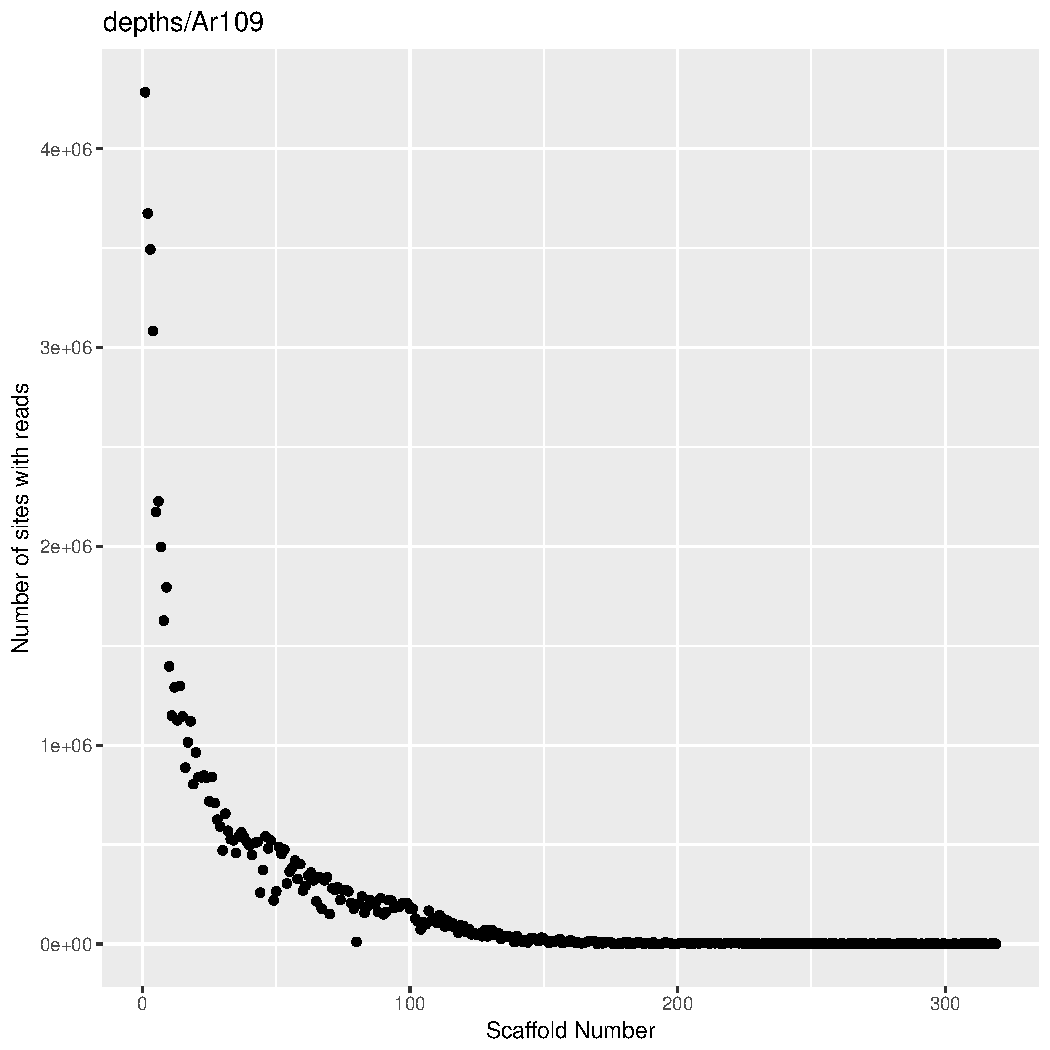
\includegraphics[angle=0,width=1.0\linewidth]{/home/thomas/Directed_Studies_Summer_2019/Armillaria_gallica_gene_analysis_tools/Reporting_documents/Figures/Ar109_collected_no_comma_count.pdf}}\\
		\begin{singlespace}
			\vspace{-0.5cm}
			\caption[Average Read Depth Per scaffold, strain Ar109.]{Average Read Depth Per scaffold and nubmer of aligned reads per scaffold, strain Ar109. (left) average read depth, (right) number of aligned reads.}\label{109avgcountgraph}
		\end{singlespace}
	\end{centering}
\end{figure}

%%%%%%%%%%%%%%%%%%%%%%%%%%%%%%%%%%%
%
%	Identifying Regions of High Read Depth
%
%%%%%%%%%%%%%%%%%%%%%%%%%%%%%%%%%%%
\section{Identifying Regions of High Read Depth}
	There were two issues with the methodology Hao used to identify regions of high read depth. The first was that if the read depth peaked over the theshold for only a few locations then it would be captured in his search. This resulted in many locations of significance ranging only a few nucleotides. The second issue was that if the region of significance dipped below the search threshold then immeadiatly rose up above then a region which should have been contigious results in two regions identified. We attempted to solve this second issue by creating out own significant read depth search program. This program searched for all locations which were five times the standard deviation above the mean read depth for that scaffold and outputted those regions. The program also allowed for a customisable \textit{grace} peroid (set to 10 locations currently) where if the read depth at a loation drops below the threshold for less than the grace peroid then the regions is treated as contigious. An example of a read depth snapshot is shown below in figure \ref{rdsnpstdevgrace}.
\begin{figure}[H]
	\begin{centering}
		\resizebox{50mm}{50mm}{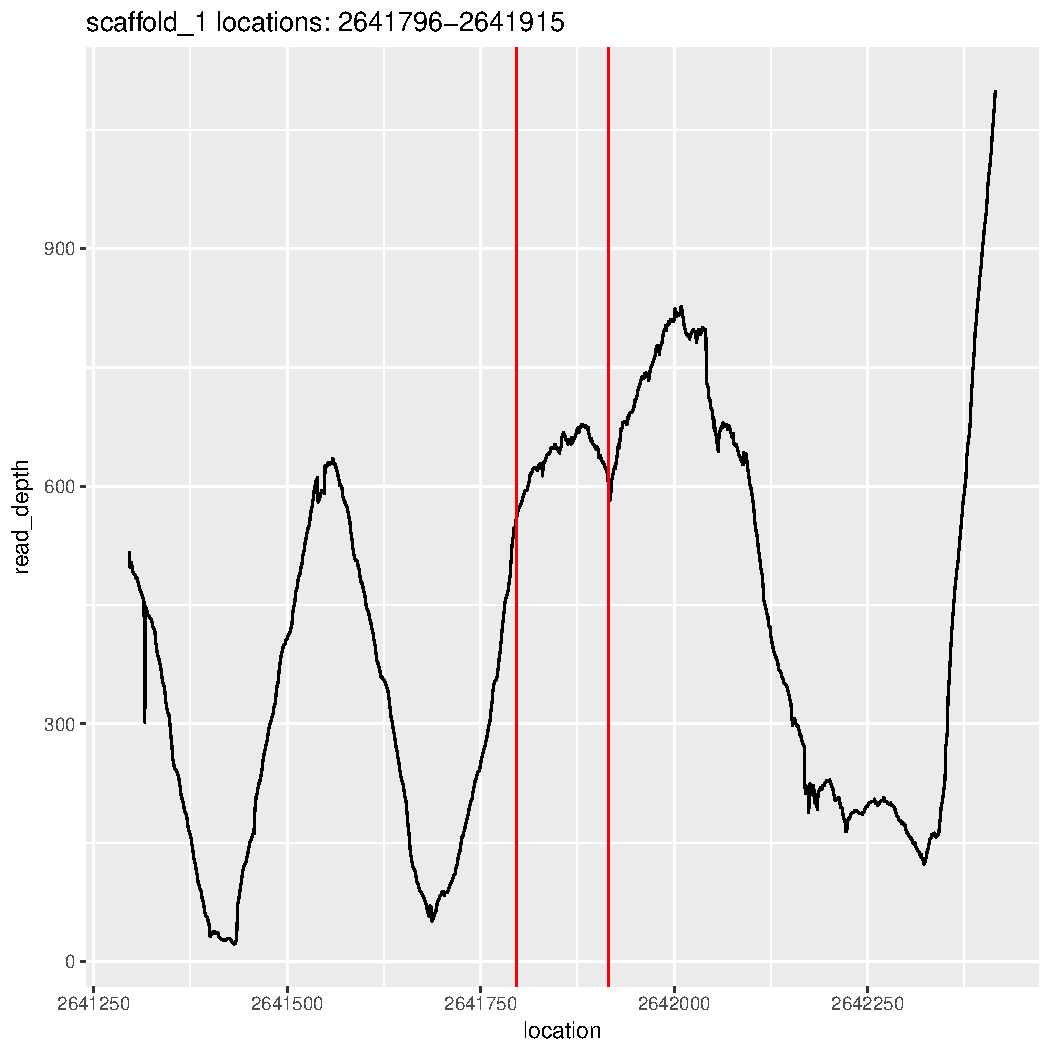
\includegraphics[angle=0,width=1.0\linewidth]{/home/thomas/Directed_Studies_Summer_2019/Armillaria_gallica_gene_analysis_tools/Reporting_documents/Figures/read_depth_snapshot_images/68_Ar109_read_depth.pdf}}
		\resizebox{50mm}{50mm}{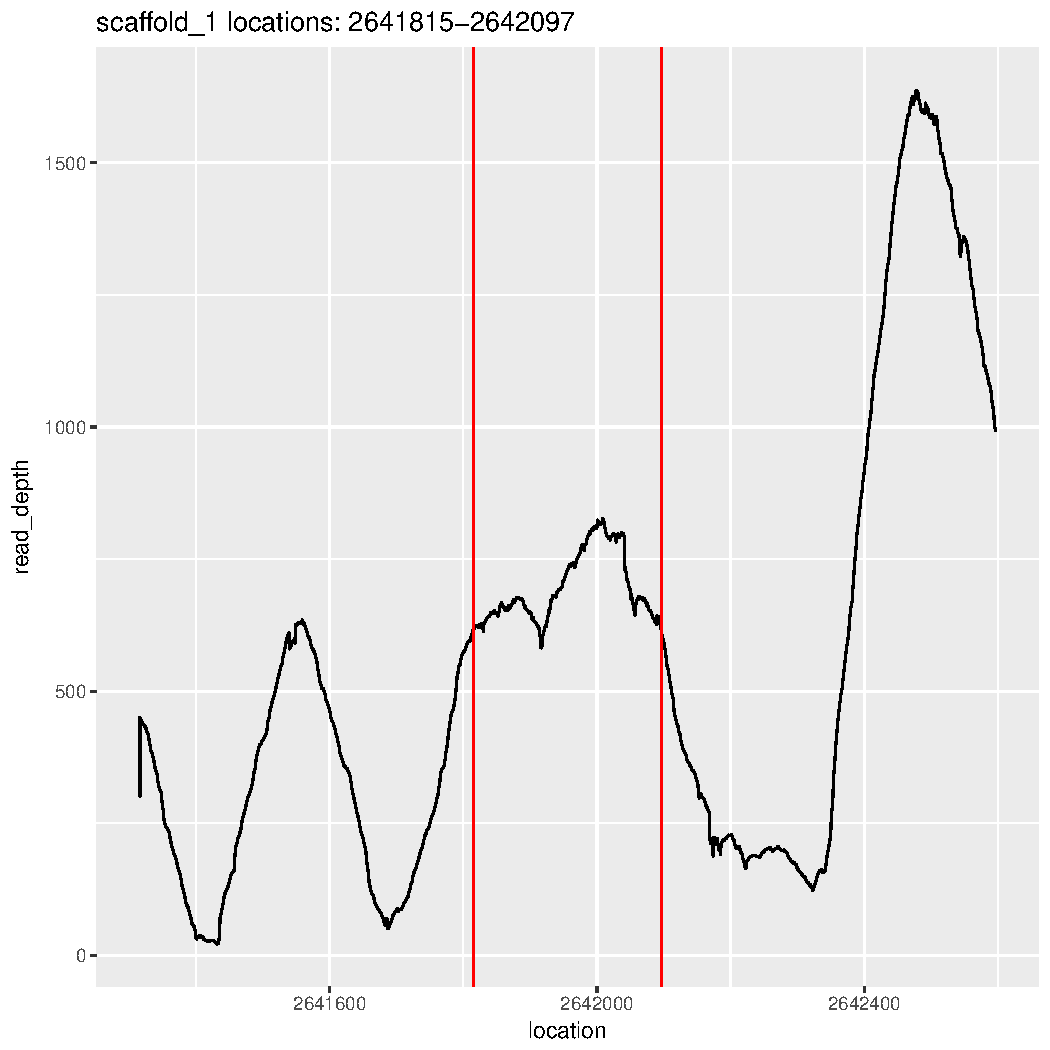
\includegraphics[angle=0,width=1.0\linewidth]{/home/thomas/Directed_Studies_Summer_2019/Armillaria_gallica_gene_analysis_tools/Reporting_documents/Figures/read_depth_snapshot_images/40_Ar109_read_depth.pdf}}\\
		\begin{singlespace}
			\vspace{-0.5cm}
			\caption[Significant Read Depth Identification Differeneces.]{Significant Read Depth Identification Differeneces. (left) Hao's method breaks the hill into two parts, (right) method with grace peroid captures intact read depth hill.}\label{rdsnpstdevgrace}
		\end{singlespace}
	\end{centering}
\end{figure}

%%%%%%%%%%%%%%%%%%%%%%%%%%%%%%%%%%%
%
%	Consensus of Aligned Reads
%
%%%%%%%%%%%%%%%%%%%%%%%%%%%%%%%%%%%
\section{Consensus of Aligned Reads}
	Between the identification of locations where there were indels and having many locations where significantlly high read depths were found it would be useful to know what the sequence at a region. To do this a series of programs were created which could take in a indexed bam file, a scaffold, a start location, and an end location. This program would then output the mode of all reads aligned within that region. 


%%%%%%%%%%%%%%%%%%%%%%%%%%%%%%%%%%%
%
%	Graphing Read Depth Across Scaffolds
%
%%%%%%%%%%%%%%%%%%%%%%%%%%%%%%%%%%%
\section{Graphing Read Depth Across Scaffolds}
	To take a birds eye view of the read depth for each scaffold, we separated each scaffold read depths into their own files and graphed the individial scaffold read depth. The scaffolds vary in size greatly, as can be seen in figure \ref{109avgcountgraph}. Shown below in figure \ref{wholescaffandhisto}are scaffolds 1 and 200 for strain Ar109 and the histograms of the read depths.

\begin{figure}[H]
	\begin{centering}

		\resizebox{110mm}{45mm}{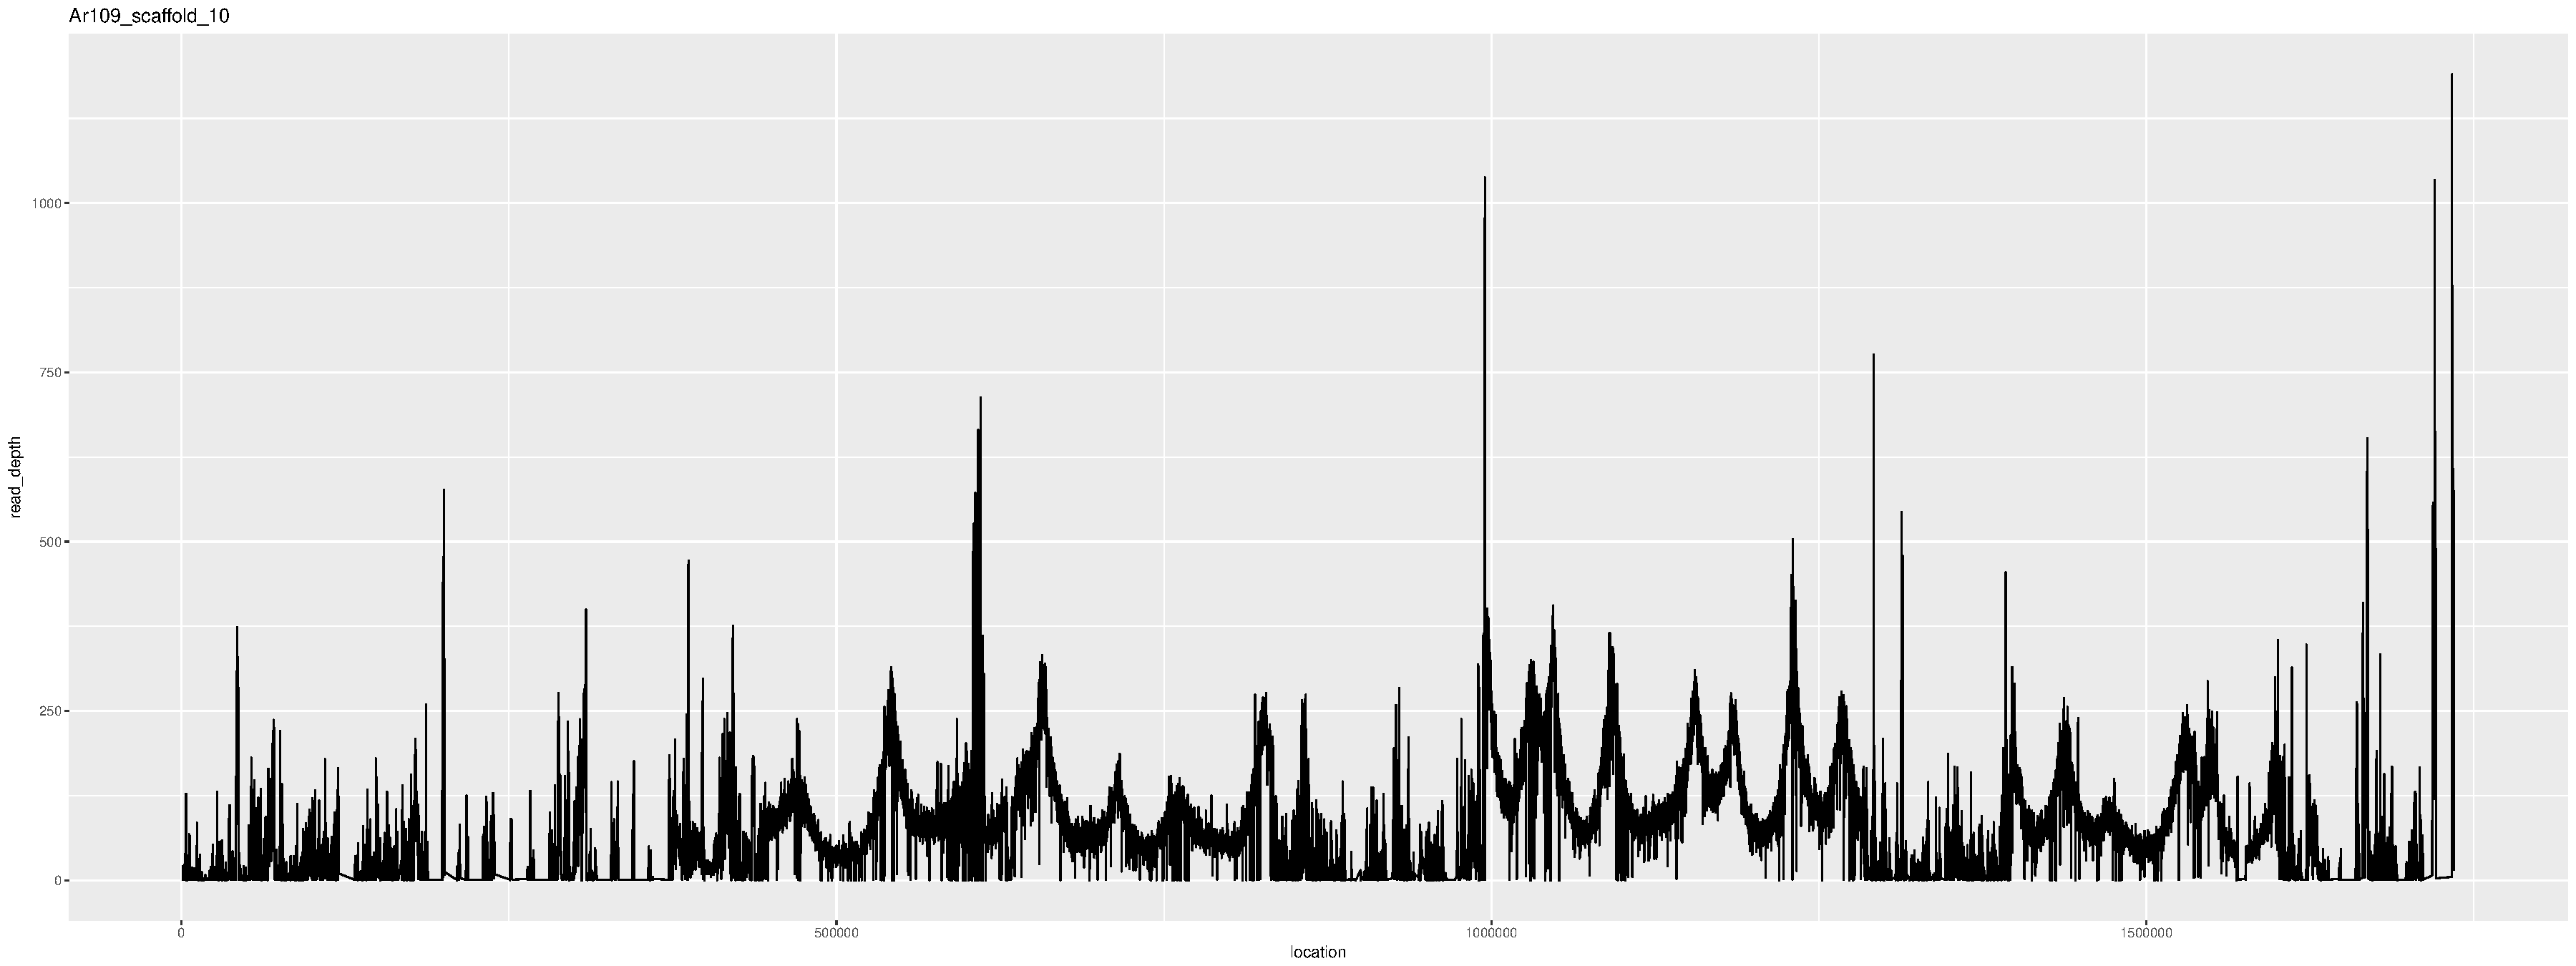
\includegraphics[angle=0,width=1.0\linewidth]{/home/thomas/Directed_Studies_Summer_2019/Armillaria_gallica_gene_analysis_tools/Reporting_documents/Figures/whole_scaffold_images/Ar109_scaffold_10_read_depth.pdf}}
		\resizebox{45mm}{45mm}{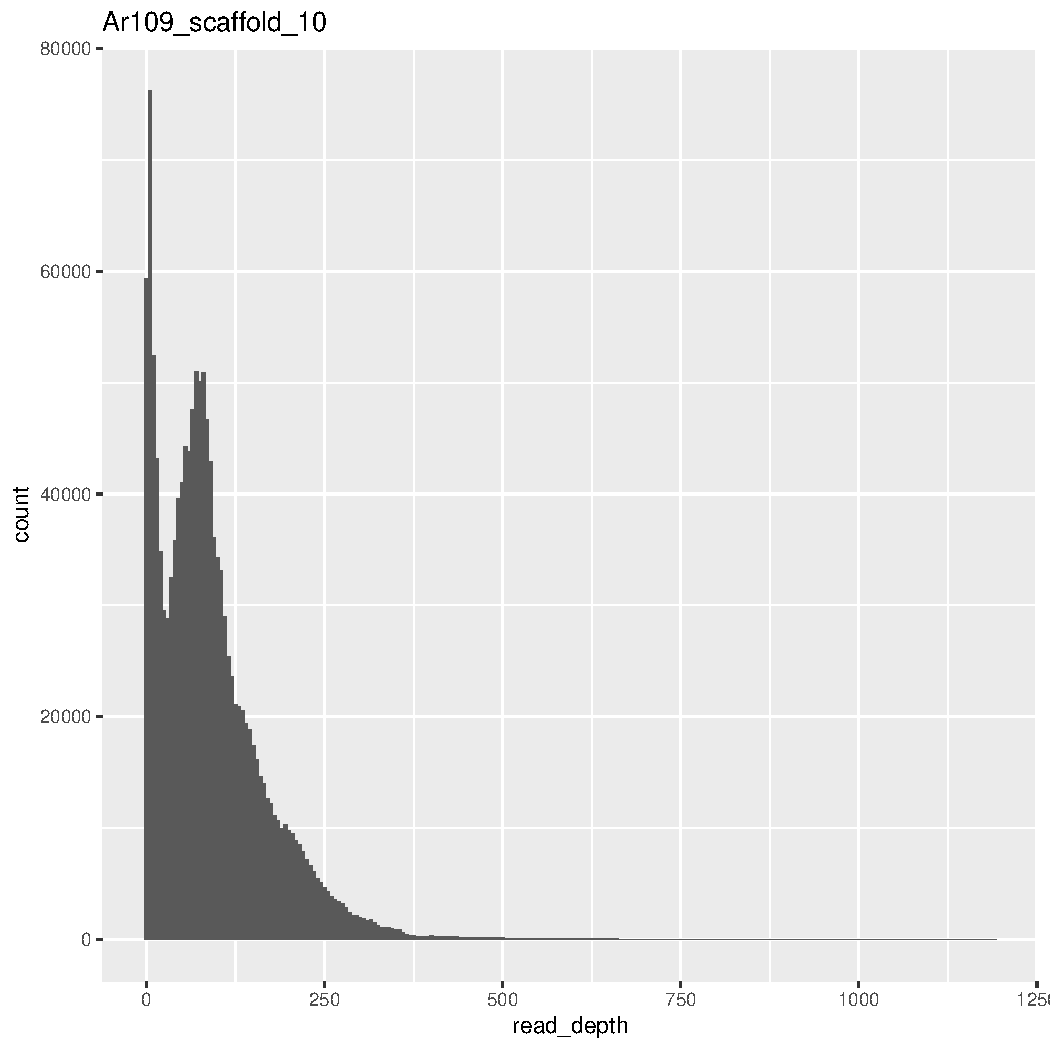
\includegraphics[angle=0,width=1.0\linewidth]{/home/thomas/Directed_Studies_Summer_2019/Armillaria_gallica_gene_analysis_tools/Reporting_documents/Figures/whole_scaffold_images/Ar109_scaffold_10_read_depth_histogram.pdf}}\\
		\resizebox{110mm}{45mm}{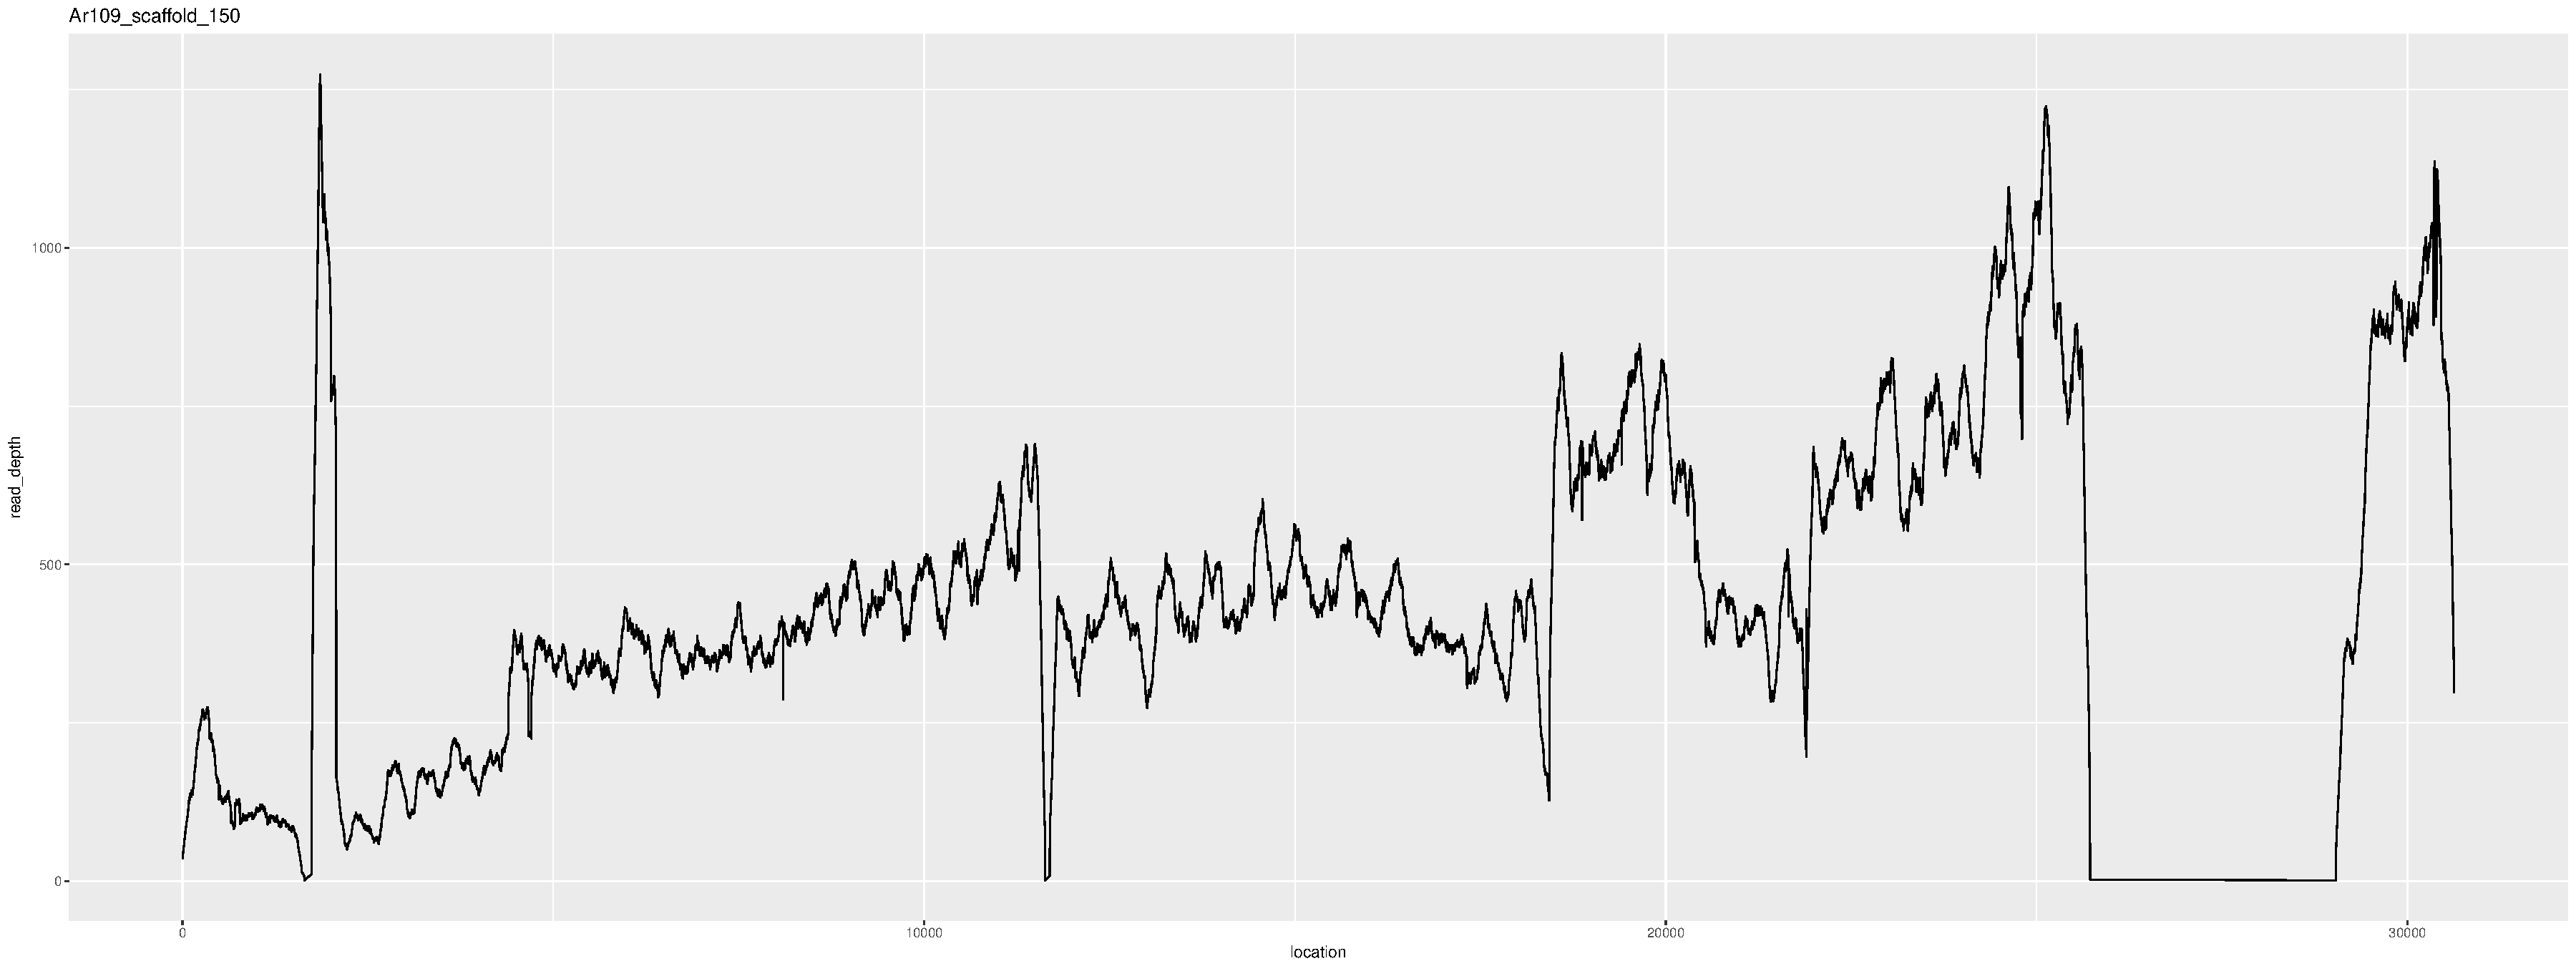
\includegraphics[angle=0,width=1.0\linewidth]{/home/thomas/Directed_Studies_Summer_2019/Armillaria_gallica_gene_analysis_tools/Reporting_documents/Figures/whole_scaffold_images/Ar109_scaffold_150_read_depth.pdf}}
		\resizebox{45mm}{45mm}{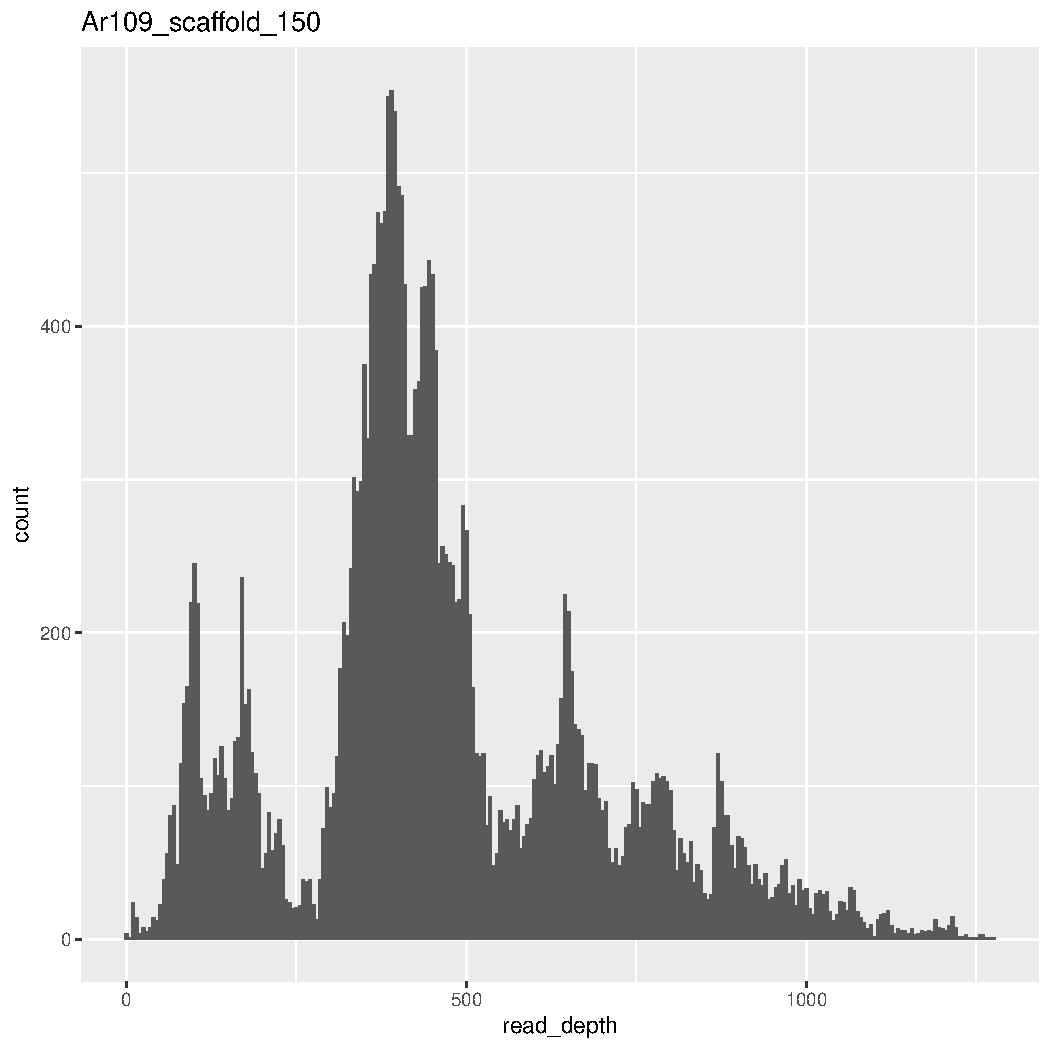
\includegraphics[angle=0,width=1.0\linewidth]{/home/thomas/Directed_Studies_Summer_2019/Armillaria_gallica_gene_analysis_tools/Reporting_documents/Figures/whole_scaffold_images/Ar109_scaffold_150_read_depth_histogram.pdf}}\\
		\begin{singlespace}
			\vspace{-0.5cm}
			\caption[Whole Scaffold Read Depth Graphs.]{Whole Scaffold Read Depth Graphs for strain Ar109. (Top left) Scaffold 10 read depth, (Top right) scaffold 10 histogram, (Bottom left) Scaffold 150 read depth, (Bottom right) scaffold 150 histogram.}\label{wholescaffandhisto}
		\end{singlespace}
	\end{centering}
\end{figure}

%%%%%%%%%%%%%%%%%%%%%%%%%%%%%%%%%%%
%
%	Read Depth Differences Between Strains
%
%%%%%%%%%%%%%%%%%%%%%%%%%%%%%%%%%%%
\section{Read Depth Differences Between Strains}
	To compare the read depths between strains we created a program which would iterate over two read depth files and output the differences in read depth at all locations. Due to the similarity of the output from this program to the input used in the program to find significant read depths we were able to perform the analysis same analysis outlined in the section on identifying regions of high read depth. These sequences could then graphed and blasted.

%%%%%%%%%%%%%%%%%%%%%%%%%%%%%%%%%%%
%
%	Assemblies
%
%%%%%%%%%%%%%%%%%%%%%%%%%%%%%%%%%%%
\section{Assemblies}
	The bam files which we were able to work with were created using reference based assembly, but the unaligned reads were stripped from the file. One of the experiments which we wanted to carry out was to create an assembly of the unaligned reads and to see how those 15 assemblies may have compared to eachother. In order to gain access to these reads we attempted new reference based assemblies using five of the 15 strains. Although these assemblies have been completed, they have not been analyzed yet due to time constraints.

	We also attempted de novo assemblies of five of the 15 fastq sequences we had. These de novo assemblies were carried out using Velvet and VelvetOptimiser, using default settings. Unfortunatly the results from these assemblies were of low quality. The largest contig was roughly 5000 bases and the total number of contigs was over 150,000. In the future we will attempt to determine why these de novo assemblies turned out so poorly.

%%%%%%%%%%%%%%%%%%%%%%%%%%%%%%%%%%%
%
%	Sequence Identification With Blastn
%
%%%%%%%%%%%%%%%%%%%%%%%%%%%%%%%%%%%
\section{Sequence Identification With Blastn}
	Making use of the identified regions of high read depth and the program which can extract sequences from the bam file we were able to use blastn to attempt to determine the function of the different notable sequences. Due to the high number of sequences we were only able to search a small fracton of the total, and the results from those searches were inconclusive. Nearly all of the sequences searched had no hits and the few that did were mainly mRNA sequences. We deteremined that there is a method to carry out multiple blastn searches quickly, although we have not yet been able to make the program needed for this function. When we can get this method working we will be able to carry out an automated blast search of any sequence we find interesting.   

%%%%%%%%%%%%%%%%%%%%%%%%%%%%%%%%%%%
%
%	Sequence Identification With Blastn
%
%%%%%%%%%%%%%%%%%%%%%%%%%%%%%%%%%%%
\section{RNA Verification of Blast Method}
	Due to the low number of sinificant blast results, we attempted to very this method of search by attempting to find a sequence which we know to be present in \textit{Armillaria Gallica}. Specifically we obtained a partial 18S rRNA sequence for the fungus \textit{Aspergillus niger} that was roughly 1700 nucltotides long, and blasted that sequence against the reference genome for \textit{Armillaria Gallica} on the joint Genome Institue Fungal Genomics Resource website. This blast returned a hit for a small region on scaffold 10 (scaffold 10:994951-995150), although this region was only 199 nucltodies in length. When we searched for this region in our scaffold snapshot graphs we were able to find that it was identified as a region of notable read depth by our system. The read depth snapshot for this range is shown in figure \ref{rdsnp18Srrna}. The total ribosomal DNA for \textit{Armillaria Gallica} should be larger than 10kb although and the 18S subunit should be larger than 3kb. We did complete a search for the entire ribosomal DNA sequence but the best we could find was a partial 28S sequence and a partial 18S/28S sequence which when blasting against the reference we found no matches. A portion of individual 28S subunit could be verified in the same method as used for the 18S subunit, but the larger 18S/28S gene could not be found. We suspect that the reference does not include the whole ribosomal DNA sequence and it may be that the ribosomal sequences present in the 15 strains of \textit{Armillaria Gallica} are contained in the unalinged reads. 
      \begin{figure}[H]
	\begin{centering}
\resizebox{50mm}{50mm}{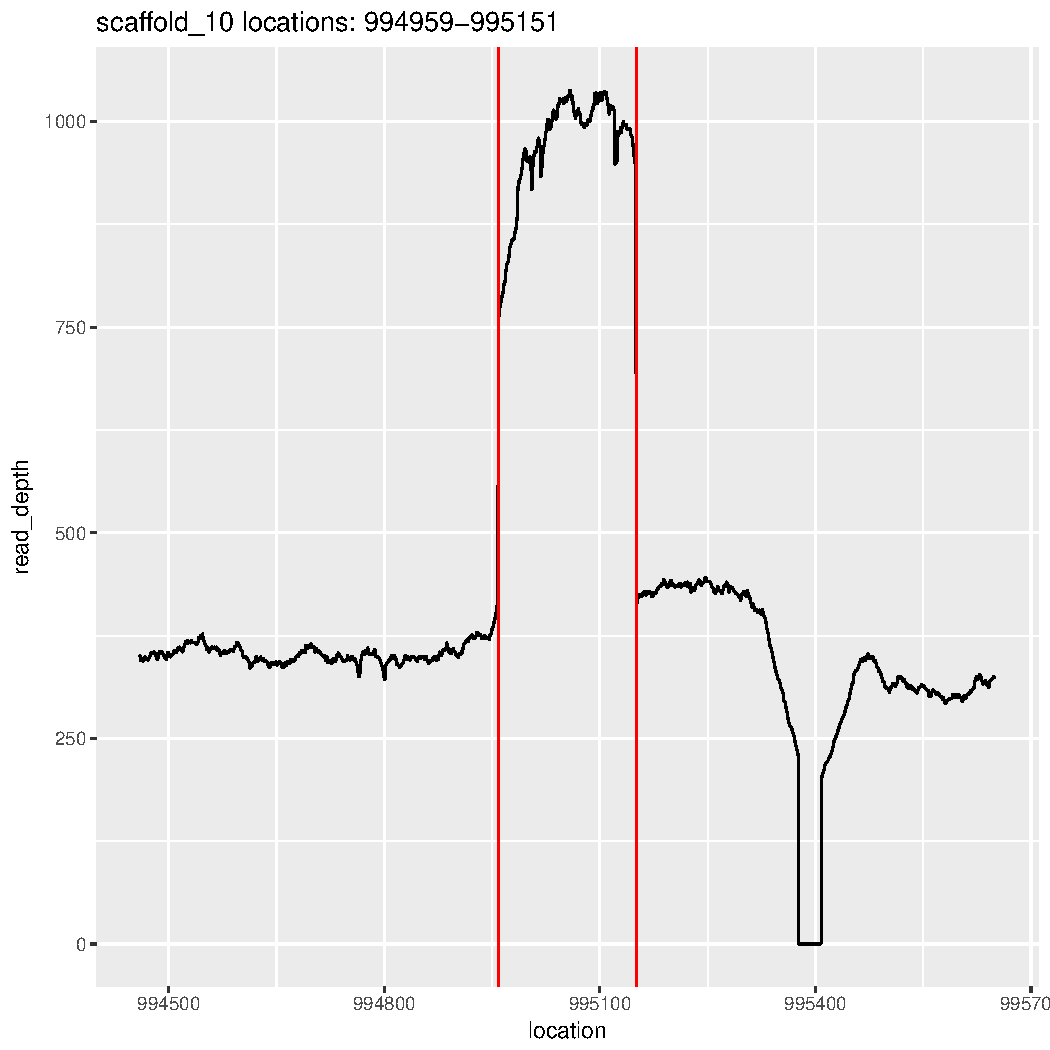
\includegraphics[angle=0,width=1.0\linewidth]{/home/thomas/Directed_Studies_Summer_2019/Armillaria_gallica_gene_analysis_tools/Reporting_documents/Figures/read_depth_snapshot_images/433_Ar109_read_depth.pdf}}
 		\begin{singlespace}
			\vspace{-0.5cm}
			\caption[Read Depth for Partial 18S Sequence.]{Read Depth for Partial 18S Sequence.}\label{rdsnp18Srrna}
		\end{singlespace}
	\end{centering}
\end{figure}
%%%%%%%%%%%%%%%%%%%%%%%%%%%%%%%%%%%
%
%	Indel Analysis
%
%%%%%%%%%%%%%%%%%%%%%%%%%%%%%%%%%%%
\section{Indel Analysis}


%%%%%%%%%%%%%%%%%%%%%%%%%%%%%%%%%%%
%
%	Future Directions
%
%%%%%%%%%%%%%%%%%%%%%%%%%%%%%%%%%%%
\section{Future Directions}
\begin{itemize}
\item Attempt to find larger indels using a different methodology
\vspace{-0.5cm}
\item Take full inventory, via blastn, of all the indels identified and the immediate regions surrounding them 
\vspace{-0.5cm}
\item Create a more robust method to search for regions of high read depth
\vspace{-0.5cm}
\item Take full inventory of all the sequences at regions of high read depth
\vspace{-0.5cm}
\item Look at the sequences which result from comparison of 
\vspace{-0.5cm}
\item Search for transposons
\vspace{-0.5cm}
\item Complete De novo assemblies and carry out many of these analyses on those
\vspace{-0.5cm}
\item Look into the reads which did not align to the reference and attempt to find any variation which may exist between the strains
\end{itemize}

\end{document}
